% siminos/chen/projectFall17/chapters/KSintro.txt    pdflatex project
% $Author: predrag $ $Date: 2021-01-22 16:12:00 -0500 (Fri, 22 Jan 2021) $


\KSe\ is one of the most studied models of
complex \spt\ dynamics in spatially extended systems.
It was formulated
independently by Kuramoto in the context of angular phase
turbulence in reaction-diffusion systems\rf{KurTsu75}, and
by Sivashinsky in the study of hydrodynamic instability of laminar
flames\rf{michsiv77}.
It also describes the instabilities of
dissipative trapped ion modes in plasmas\rf{laquey74} and the
flow of a viscous liquid film down a vertical wall\rf{ShSi82}.
Its one\dmn\ form is frequently written as
\begin{equation}
  u_t+\frac{1}{2}(u^2)_x+u_{xx}+u_{xxxx}=0\,,\; x\in [0,L]
  \label{eq:ks}
\end{equation}
defined on a periodic domain $u(x, t) = u(x+L, t)$.
In the combustion formulation, $u(x, t)$ represents the
flame front velocity. Everyday experience tells us that a candle flame
flickers and its shape changes quite often, without any exterior influence.
Therefore, \KSe\ is expected to exhibit chaotic behaviors.
\refFig{fig:KS_L100200} displays its \spt\ profiles with
domain size $L=100$ and $200$ respectively. Recurrent patterns appear not
only along the temporal axis but also along the spatial axis. This \spt\
chaotic behavior is also observed in other spatially-extended dynamical
systems such as \cGLe\rf{SPScgl92}.
At the same time, \reffig{fig:KS_L100200} provides coarse information about
the time and length scale of this ``dimensionless'' system.
In all our simulations, we set $L = 22$, which is large enough to exhibit
complex \spt\ chaotic dynamics{\rf{SCD07}}.

\begin{figure}
  \centering
  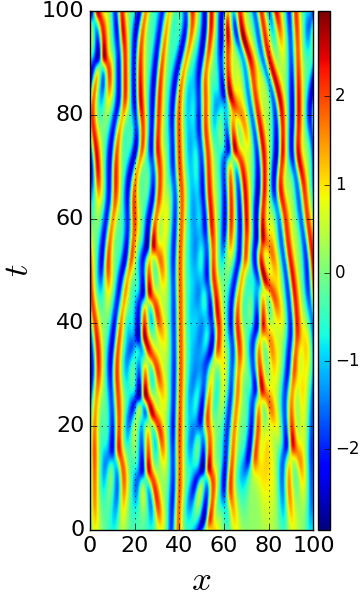
\includegraphics[height=0.35\textheight]{KS_L100N256}
  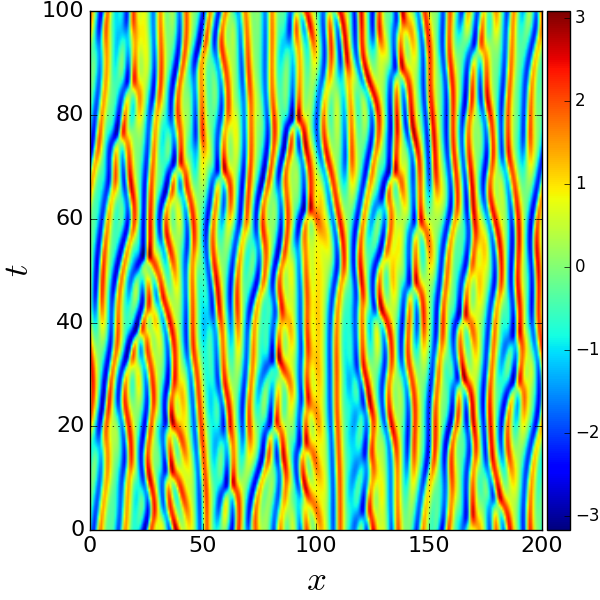
\includegraphics[height=0.35\textheight]{KS_L200N256}
  \caption[\Spt\ plots of the one\dmn\ \KSe\ for $L=100$ and $200$.]{
    Simulations of the one\dmn\ \KSe\ for domain size $L=100, 200$ respectively with random initial
    conditions. The color represents the magnitude of $u(x, t)$.
  }
  \label{fig:KS_L100200}
\end{figure}

To summarize, the form of the \KSe\ \refeq{eq:ks} on a periodic domain in one
space dimension that we use in this report is
\beq
    u_\zeit =  - u u_\conf
    -u_{\conf \conf}-u_{\conf \conf \conf \conf}
\,,\qquad
    x\in [0,L]
\,,
\ee{ACe-ks}
where subscripts denote partial derivatives.